\documentclass[aspectratio=169,10pt]{beamer}
\usepackage[utf8]{inputenc}
\usepackage[T1]{fontenc}
\usepackage{amsmath,amssymb}
\usepackage{graphicx}
\usepackage{booktabs,array}

\definecolor{Ink}{HTML}{172B3A}
\definecolor{Navy}{HTML}{183B56}
\definecolor{Teal}{HTML}{087E8B}
\definecolor{Gold}{HTML}{D99A2B}
\definecolor{Mist}{HTML}{EEF4F6}
\definecolor{Alert}{HTML}{B23A48}

\usetheme{default}
\setbeamertemplate{navigation symbols}{}
\setbeamertemplate{itemize item}{\color{Teal}$\blacktriangleright$}
\setbeamertemplate{itemize subitem}{\color{Gold}$\bullet$}
\setbeamercolor{normal text}{fg=Ink,bg=white}
\setbeamercolor{frametitle}{fg=white,bg=Navy}
\setbeamercolor{structure}{fg=Teal}
\setbeamerfont{frametitle}{series=\bfseries,size=\large}
\setbeamersize{text margin left=0.55cm,text margin right=0.55cm}
\setbeamertemplate{footline}{%
  \leavevmode\hbox{%
  \begin{beamercolorbox}[wd=.78\paperwidth,ht=2.6ex,dp=1.1ex,leftskip=.55cm]{author in head/foot}%
    \color{Navy}\scriptsize Repository 4 deep dive \enspace\textcolor{Teal}{|}\enspace
    Acemoglu, Kong \& Ozdaglar (2026)
  \end{beamercolorbox}%
  \begin{beamercolorbox}[wd=.22\paperwidth,ht=2.6ex,dp=1.1ex,rightskip=.55cm plus1fil]{date in head/foot}%
    \color{Navy}\scriptsize\hfill\insertframenumber/\inserttotalframenumber
  \end{beamercolorbox}}}

\newcommand{\paperlabel}{\textcolor{Navy}{\scriptsize\bfseries PAPER RESULT}}
\newcommand{\extlabel}{\textcolor{Alert}{\scriptsize\bfseries OUR PROPOSED EXTENSION --- NOT IN THE PAPER}}
\newcommand{\interpretlabel}{\textcolor{Gold}{\scriptsize\bfseries OUR INTERPRETATION}}
\newcommand{\softbox}[1]{\begin{beamercolorbox}[rounded=true,sep=.6em]{block body}#1\end{beamercolorbox}}
\setbeamercolor{block body}{fg=Ink,bg=Mist}

\begin{document}

% 1
\begin{frame}[plain]
  \vspace{.7cm}
  {\color{Teal}\rule{1.8cm}{3pt}}\par
  \vspace{.4cm}
  {\color{Navy}\fontsize{25}{29}\selectfont\bfseries
    AI, Human Cognition and\\ Knowledge Collapse\par}
  \vspace{.3cm}
  {\large Acemoglu, Kong \& Ozdaglar (2026)}\par
  \vspace{.5cm}
  NBER Working Paper 34910 \enspace\textcolor{Teal}{|}\enspace February 2026\par
  \vspace{.3cm}
  {\color{Gold}\bfseries Deep-dive and oral-exam backup}\par
  \vfill
  \href{https://github.com/carlosgomezp28/ai-04-acemoglu}{%
    \color{Teal}\texttt{github.com/carlosgomezp28/ai-04-acemoglu}}
  \vspace{.35cm}
\end{frame}

% 2
\begin{frame}{Research question and mechanism}
  \paperlabel
  \vspace{.15cm}

  \begin{beamercolorbox}[rounded=true,sep=.75em]{block body}
    \centering\large How does agentic AI change human learning incentives and
    the long-run stock of collective knowledge?
  \end{beamercolorbox}

  \vspace{.4cm}
  \begin{columns}[T,onlytextwidth]
    \begin{column}{.30\textwidth}
      \centering
      {\color{Navy}\bfseries HUMAN EFFORT}\par
      \vspace{.15cm}
      private context signal\par
      {\color{Teal}$+$}\par
      thin public signal
    \end{column}
    \begin{column}{.08\textwidth}
      \centering\vspace{.45cm}{\color{Gold}\Large$\Longrightarrow$}
    \end{column}
    \begin{column}{.26\textwidth}
      \centering
      {\color{Navy}\bfseries TWO RETURNS}\par
      \vspace{.15cm}
      private task success\par
      {\color{Teal}$+$}\par
      future public knowledge
    \end{column}
    \begin{column}{.08\textwidth}
      \centering\vspace{.45cm}{\color{Gold}\Large$\Longleftarrow$}
    \end{column}
    \begin{column}{.26\textwidth}
      \centering
      {\color{Navy}\bfseries AGENTIC AI}\par
      \vspace{.15cm}
      context-specific precision\par
      substitutes for the\par
      private motive to learn
    \end{column}
  \end{columns}

  \vspace{.5cm}
  \softbox{\small The externality is the hinge: short-lived agents receive the
  private return from learning, but do not internalize the knowledge inherited by
  later cohorts.}
\end{frame}

% 3
\begin{frame}{States and information structure}
  \paperlabel
  \vspace{.12cm}
  \begin{columns}[T,onlytextwidth]
    \begin{column}{.48\textwidth}
      \textbf{Latent states}
      \begin{align*}
        \theta_{t+1}&=\theta_t+\varepsilon_t,
        &\varepsilon_t&\sim\mathcal N(0,\Sigma^2),\\
        \theta_{i,t}&\overset{\rm iid}{\sim}\mathcal N(0,\sigma^2).
      \end{align*}
      \textbf{Signals}
      \begin{align*}
        s^H_{i,t}&\sim\mathcal N\!\left(\theta_{i,t},(\lambda_Ie_{i,t})^{-1}\right),\\
        s^A_{i,t}&\sim\mathcal N\!\left(\theta_{i,t},\tau_A^{-1}\right),\\
        s^C_t&\sim\mathcal N\!\left(\theta_t,(\lambda_G I e_t)^{-1}\right).
      \end{align*}
    \end{column}
    \begin{column}{.49\textwidth}
      \textbf{Posterior precisions}
      \[
        X_t=\operatorname{Var}(\theta_t\mid\mathcal I_t)^{-1},
      \]
      \[
        \boxed{Y_{i,t}=\sigma^{-2}+\lambda_Ie_{i,t}+\tau_A}.
      \]
      \begin{beamercolorbox}[rounded=true,sep=.65em]{block body}
      \small
      $X_t$ is inherited, public, general knowledge.\par\medskip
      $Y_{i,t}$ combines prior precision, human learning, and the agentic-AI
      recommendation for the current context.
      \end{beamercolorbox}
    \end{column}
  \end{columns}
\end{frame}

% 4
\begin{frame}{Production technology}
  \paperlabel
  \vspace{.12cm}
  \begin{columns}[T,onlytextwidth]
    \begin{column}{.56\textwidth}
      \textbf{Four task outcomes, re-parameterized}
      \begin{align*}
        \Delta_G&=f(1,0)-f(0,0),\\
        \Delta_I&=f(0,1)-f(0,0),\\
        \Delta_X&=f(1,1)-f(1,0)-f(0,1)+f(0,0).
      \end{align*}
      The normalization $f(1,1)-f(0,0)=1$ gives
      \[
        \Delta_G+\Delta_I+\Delta_X=1.
      \]
    \end{column}
    \begin{column}{.41\textwidth}
      \begin{beamercolorbox}[rounded=true,sep=.8em]{alerted text}
        \centering\textbf{Assumption 1}
        \[
          \boxed{\Delta_I=0,\qquad \Delta_X>0.}
        \]
      \end{beamercolorbox}
      \vspace{.25cm}
      \small
      $\Delta_I=0$ is strong: correct context-specific knowledge has no
      incremental productive value unless general knowledge is also correct.

      \vspace{.2cm}
      $\Delta_X>0$ supplies strict complementarity; $\Delta_G$ may be positive.
    \end{column}
  \end{columns}
\end{frame}

% 5
\begin{frame}{Static expected utility}
  \paperlabel
  \vspace{.12cm}
  Let $p_G=G(X)$ and $p_I=G(Y)$ be the two Gaussian success probabilities.
  The four production outcomes imply the accounting identity
  \[
  \mathbb E[f]
   =f_{00}+\Delta_Gp_G+\Delta_Ip_I+\Delta_Xp_Gp_I.
  \]

  \vspace{.15cm}
  Under the paper's maintained $\Delta_I=0$,
  \begin{beamercolorbox}[rounded=true,sep=.7em]{block body}
  \[
  \boxed{
  U(e;X,\tau_A)=f_{00}+\Delta_GG(X)+\Delta_XG(X)G(Y)
  -\frac{e^\alpha}{\alpha}}
  \]
  \[
    Y=\sigma^{-2}+\lambda_Ie+\tau_A,\qquad \alpha>1.
  \]
  \end{beamercolorbox}

  \vspace{.2cm}
  \small The individual treats $X$ as given: her infinitesimal public-learning
  contribution benefits future cohorts and is not privately internalized.
\end{frame}

% 6
\begin{frame}{First-order condition and uniqueness}
  \paperlabel
  \vspace{.12cm}
  \[
  U_e=\underbrace{\Delta_XG(X)\lambda_Ig(Y)}_{\text{marginal information benefit}}
       -\underbrace{e^{\alpha-1}}_{\text{marginal effort cost}}.
  \]
  \[
    \boxed{\Delta_XG(X)\lambda_Ig(\sigma^{-2}+\lambda_Ie+\tau_A)
    =e^{\alpha-1}}
  \]

  \vspace{.2cm}
  \begin{columns}[T,onlytextwidth]
    \begin{column}{.49\textwidth}
      \softbox{\small Since $g$ is decreasing, marginal benefit weakly falls
      with $e$. Since $\alpha>1$, marginal cost strictly rises. Their crossing is
      unique and finite.}
    \end{column}
    \begin{column}{.49\textwidth}
      \begin{beamercolorbox}[rounded=true,sep=.6em]{alerted text}
      \small At $X=0$, $G(0)=0$: the information benefit vanishes and the paper's
      unique best response is $e(0,\tau_A)=0$.
      \end{beamercolorbox}
    \end{column}
  \end{columns}
\end{frame}

% 7
\begin{frame}{Observation 1: general knowledge}
  \paperlabel
  \vspace{.15cm}
  \[
  U_e=\Delta_XG(X)\lambda_Ig(Y)-e^{\alpha-1}.
  \]
  Differentiate the marginal return to effort with respect to public precision:
  \[
    \boxed{U_{eX}=\Delta_X\lambda_Ig(X)g(Y)>0.}
  \]

  \vspace{.25cm}
  \begin{beamercolorbox}[rounded=true,sep=.75em]{block body}
    \textbf{Conditions for the strict sign:}
    \[
      \Delta_X>0,\quad\lambda_I>0,\quad X>0,\quad Y>0,
      \qquad g(X)>0,\quad g(Y)>0.
    \]
  \end{beamercolorbox}

  \vspace{.25cm}
  \small More general knowledge makes context-specific evidence more useful;
  that raises the marginal return to acquiring one's own signal.
\end{frame}

% 8
\begin{frame}{Observation 1: agentic AI}
  \paperlabel
  \vspace{.15cm}
  Since $\partial Y/\partial\tau_A=1$,
  \[
    \boxed{U_{e\tau_A}=\Delta_XG(X)\lambda_Ig'(Y)<0.}
  \]

  \vspace{.25cm}
  \begin{beamercolorbox}[rounded=true,sep=.75em]{block body}
    \textbf{Conditions for the strict sign:}
    \[
      \Delta_X>0,\quad \lambda_I>0,\quad X>0,\quad Y>0,
      \qquad G(X)>0,\quad g'(Y)<0.
    \]
  \end{beamercolorbox}

  \vspace{.35cm}
  \begin{columns}[c,onlytextwidth]
    \begin{column}{.30\textwidth}\centering more AI precision $\tau_A$\end{column}
    \begin{column}{.08\textwidth}\centering{\color{Gold}\Large$\Longrightarrow$}\end{column}
    \begin{column}{.27\textwidth}\centering lower marginal gain from self-acquired precision\end{column}
    \begin{column}{.08\textwidth}\centering{\color{Gold}\Large$\Longrightarrow$}\end{column}
    \begin{column}{.25\textwidth}\centering lower human effort\end{column}
  \end{columns}
\end{frame}

% 9
\begin{frame}{The welfare trap}
  \paperlabel
  \vspace{.12cm}
  \begin{columns}[T,onlytextwidth]
    \begin{column}{.45\textwidth}
      \begin{beamercolorbox}[rounded=true,sep=.7em]{block body}
      \textbf{STATIC --- hold $X$ fixed}
      \[
        \tau_A\uparrow\quad\Rightarrow\quad G(Y)\uparrow
      \]
      More accurate advice raises the private value of the current decision.
      \end{beamercolorbox}
    \end{column}
    \begin{column}{.53\textwidth}
      \begin{beamercolorbox}[rounded=true,sep=.7em]{alerted text}
      \textbf{DYNAMIC --- equilibrium feedback}
      \[
        \tau_A\uparrow\Rightarrow e_t\downarrow
        \Rightarrow X_{t+1}\downarrow.
      \]
      Less human learning weakens the public knowledge inherited by later cohorts.
      \end{beamercolorbox}
    \end{column}
  \end{columns}

  \vspace{.35cm}
  \small Under Assumption 2, $\sigma^{-2}\ge\sqrt2-1$:
  \begin{itemize}\small
    \item if $\alpha-1>1/4$, Proposition 10 gives a finite welfare peak
      $\tau_A^*$ (possibly zero);
    \item if $\alpha-1<1/4$, Proposition 11 gives the analogous peak below the
      collapse threshold $\tau_A^c$, and sufficiently accurate AI can eliminate
      the high-knowledge steady state.
  \end{itemize}
  \centering\textbf{A positive static AI effect does not imply monotone long-run welfare.}
\end{frame}

% 10
\begin{frame}{What Section 5 relaxes}
  \paperlabel
  \vspace{.12cm}
  \footnotesize
  \renewcommand{\arraystretch}{1.5}
  \begin{tabular}{@{}>{\raggedright\arraybackslash}p{.24\textwidth}
                      >{\raggedright\arraybackslash}p{.31\textwidth}
                      >{\raggedright\arraybackslash}p{.39\textwidth}@{}}
    \toprule
    \textbf{Section} & \textbf{Baseline object changed} & \textbf{Main qualitative consequence} \\
    \midrule
    5.1 AI-enhanced aggregation
      & Fixed $I$ becomes $I(\tau_A)=I_0+\exp(\eta\tau_A)$.
      & Substitution versus aggregation. If $\eta<1/[2(\alpha-1)]$, the high
        state still tends to zero as $\tau_A\to\infty$. \\
    5.2 Synthetic data
      & Add exogenous public precision $\tau_{\rm syn}\ge0$.
      & $\tau_{\rm syn}>0\Rightarrow F_{\rm syn}(0)>0$: the low state is
        strictly positive. \\
    5.3 Imperfect separability
      & Public precision scales with $e^\beta$ rather than $e$.
      & For $\beta>0$, baseline logic persists; the stability cutoff becomes
        $\alpha-1<\beta/4$. \\
    \bottomrule
  \end{tabular}

  \vspace{.28cm}
  \centering\textbf{All three extensions change information creation or aggregation.}
\end{frame}

% 11
\begin{frame}{What the paper never relaxes}
  \paperlabel
  \vspace{.2cm}
  \begin{beamercolorbox}[rounded=true,sep=1em]{alerted text}
    \centering\Large
    \[\boxed{\Delta_I=0,\qquad\Delta_X>0}\]
  \end{beamercolorbox}

  \vspace{.45cm}
  \begin{columns}[T,onlytextwidth]
    \begin{column}{.47\textwidth}
      \textbf{Section 5 changes}
      \begin{itemize}\small
        \item aggregation capacity $I$;
        \item exogenous public precision $\tau_{\rm syn}$;
        \item mapping from effort into public signals, $e^\beta$.
      \end{itemize}
    \end{column}
    \begin{column}{.49\textwidth}
      \textbf{Section 5 does not change}
      \begin{itemize}\small
        \item the task-production function $f$;
        \item zero standalone value of context-specific success;
        \item strict production complementarity.
      \end{itemize}
    \end{column}
  \end{columns}

  \vspace{.25cm}
  \centering{\color{Alert}\bfseries This is the production-side trap.}
\end{frame}

% 12
\begin{frame}{Proposed extension: standalone context-specific value}
  \extlabel
  \vspace{.12cm}
  \begin{columns}[T,onlytextwidth]
    \begin{column}{.56\textwidth}
      \textbf{Four-outcome expected payoff}
      \[
      \boxed{\begin{aligned}
      U={}&f_{00}+\Delta_GG(X)+\Delta_IG(Y)\\
          &+\Delta_XG(X)G(Y)-\frac{e^\alpha}{\alpha}.
      \end{aligned}}
      \]
      \small The new term $\Delta_IG(Y)$ makes correct context-specific
      knowledge productive even if general knowledge is wrong.
    \end{column}
    \begin{column}{.41\textwidth}
      \textbf{Assumptions}
      \[
      \Delta_I>0,\qquad \Delta_X>0,
      \]
      \[
      \Delta_G=1-\Delta_I-\Delta_X\ge0.
      \]
      Define
      \[
        B(X)=\Delta_I+\Delta_XG(X)>0.
      \]
      Then the modified FOC is
      \[
        \boxed{B(X)\lambda_Ig(Y)=e^{\alpha-1}}.
      \]
    \end{column}
  \end{columns}
\end{frame}

% 13
\begin{frame}{Baseline versus extension at $X=0$}
  \begin{columns}[T,onlytextwidth]
    \begin{column}{.46\textwidth}
      \paperlabel
      \vspace{.12cm}
      \begin{beamercolorbox}[rounded=true,sep=.75em]{block body}
      \centering
      $\Delta_I=0$ and $G(0)=0$
      \[
        \Rightarrow\quad U_e=-e^{\alpha-1}
        \quad\Rightarrow\quad e^*(0,\tau_A)=0.
      \]
      Hence the paper's transition satisfies $F(0)=0$.
      \end{beamercolorbox}
    \end{column}
    \begin{column}{.52\textwidth}
      \extlabel
      \vspace{.12cm}
      \begin{beamercolorbox}[rounded=true,sep=.7em]{alerted text}
      \centering
      $\Delta_I>0$, $\lambda_I>0$, $\alpha>1$, finite precisions
      \[
        \Rightarrow\quad e^*(0,\tau_A)>0.
      \]
      If also $\lambda_G>0$, $I>0$, and $0\le\Sigma^2<\infty$,
      \[
        \boxed{F_{\Delta_I}(0)=
        \left[(\lambda_G I e^*_0)^{-1}+\Sigma^2\right]^{-1}>0.}
      \]
      \end{beamercolorbox}
    \end{column}
  \end{columns}

  \vspace{.35cm}
  \softbox{\centering\bfseries Exact zero public knowledge is no longer a fixed
  point for finite AI precision. Severe low-knowledge outcomes may remain.}
\end{frame}

% 14
\begin{frame}{Numerical illustration and compiled Lean checks}
  \extlabel
  \vspace{.08cm}
  \begin{columns}[T,onlytextwidth]
    \begin{column}{.40\textwidth}
      \textbf{Audited calibration}
      \scriptsize
      \[
      \alpha=2,\quad \lambda_I=\lambda_G=I=\Sigma^2=1,
      \]
      \[
      \sigma^{-2}=0.5,\quad \Delta_I=0.25,
      \]
      \[
      \Delta_X=0.5,\quad \Delta_G=0.25.
      \]
      \renewcommand{\arraystretch}{1.18}
      \begin{tabular}{@{}ccc@{}}
        \toprule $X$ & $\tau_A$ & $e^*$ \\
        \midrule 0 & 0 & 0.09591 \\
        0.25 & 0 & 0.15653 \\
        0 & 2 & 0.01785 \\
        \bottomrule
      \end{tabular}
      \[
        \boxed{F(0)\approx0.08752>0.}
      \]
    \end{column}
    \begin{column}{.58\textwidth}
      \textbf{Compiled Mathlib verification}
      \begin{beamercolorbox}[rounded=true,sep=.5em]{block body}
      \footnotesize
      \textbf{PAPER}
      \begin{itemize}\footnotesize
        \item general-knowledge / effort sign;
        \item AI / effort sign.
      \end{itemize}
      \textbf{OUR EXTENSION}
      \begin{itemize}\footnotesize
        \item positive $B(X)$ and positive boundary marginal benefit;
        \item $F_{\Delta_I}(0)>0$ under added positivity assumptions.
      \end{itemize}
      \scriptsize Exact theorem names: \texttt{lean/Main.lean}
      \end{beamercolorbox}

      \vspace{.08cm}
      \scriptsize\textbf{Lean does NOT formalize} Gaussian conjugacy/derivatives,
      the optimization problem, equilibrium, or the full dynamic model.
    \end{column}
  \end{columns}
\end{frame}

% 15
\begin{frame}{Where I did not believe AI: final audit}
  \begin{columns}[T,onlytextwidth]
    \begin{column}{.47\textwidth}
      \centering
      \includegraphics[page=3,width=.94\linewidth,trim=22 355 22 18,clip]{../hand/extension-derivation.pdf}
      \par
      {\tiny Handwritten audit, p.~3}
    \end{column}
    \begin{column}{.51\textwidth}
      \extlabel
      \vspace{.08cm}
      \begin{beamercolorbox}[rounded=true,sep=.55em]{alerted text}
      \centering\scriptsize\textbf{INITIAL CLAIM}
      \[
        \Delta_I>0\Rightarrow\text{knowledge collapse is eliminated.}
      \]
      {\color{Alert}\bfseries AUDIT: TOO STRONG.}
      \end{beamercolorbox}

      \vspace{.1cm}
      \begin{beamercolorbox}[rounded=true,sep=.55em]{block body}
      \centering\scriptsize\textbf{CORRECTED CONCLUSION}
      \[
        \boxed{\Delta_I>0\Rightarrow F_{\Delta_I}(0)>0}
      \]
      \scriptsize under the relevant static and public-learning conditions.
      \end{beamercolorbox}

      \vspace{.05cm}
      \scriptsize Exact zero disappears, but low positive states, multiplicity,
      path dependence, and welfare loss may remain.

      \vspace{.04cm}
      \scriptsize\textbf{Synthetic data:} exogenous public precision; our
      mechanism: endogenous human effort.
    \end{column}
  \end{columns}

  \vspace{.05cm}
  \begin{beamercolorbox}[rounded=true,sep=.4em]{alerted text}
  \interpretlabel\quad
  \scriptsize The paper's collapse mechanism is robust to many information-side
  extensions, but its exact zero state depends critically on assuming that
  context-specific knowledge has no standalone productive value.
  \end{beamercolorbox}
\end{frame}

\end{document}
